%\documentclass[11pt]{article}
%\input{header_old.tex}
%\usepackage[none]{hyphenat} 
%\usepackage{tikz}
%\usepackage{pgfplots}
%
%\newcommand{\Course}{MATH 1331 (Cole)}
%\newcommand{\Year}{2023}
%\newcommand{\Qtr}{Fall }
%
%\renewcommand{\myTitle}{\Course}
%
%\renewcommand{\mySubTitle}{Test 1 Study Guide - \Qtr \Year}
%
%\lhead{{\Large \myTitle}}
%\chead{{\Large \textbf{Test 1 Review Problems}}}
%\rhead{{\LARGE \Qtr \Year}}
%\rfoot{\tiny Review problem questions and format are inspired by problems from Stewart's \textit{Essential Calculus, Early Transcendentals}, 2nd. Edition}
%\lfoot{}
%
%%\vspace*{-.5in}
%
%
%\begin{document}

% Instructions to change to html version:
% Comment out:
%  minipage, multicols,columnbreak, mathbf, hrule
% Replace all: \begin{minipage}% %%\end{minipage} %%%%\begin{mulicols}  %%%%\end{mulicols}  %%%\columnbreak % %%%\begin{framed} %%%%\end{framed} %%%%\hrule
% Search for \mathbf
% Replace \\] with \[ and \) with \(
% Enclose graphics in figure environments and add captions
% Re-tag \df environments as sections, subsections, etc.
% Command Line Code to Create html version:
%First: pdflatex -shell-escape filename.tex                                   
%Second, for each figure: inkscape "filename-figure1.pdf" -o "filename-figure1.png"
% Third: htlatex filename.tex "ht5mjlatex.cfg, charset=utf-8" " -cunihtf -utf8"


\documentclass[10pt]{article}

%\usepackage{tikz, pgf,pgfplots,wasysym,array}
%\usepackage{wasysym,array}

\usepackage{amsmath,amssymb}

\ifdefined\HCode
  \def\pgfsysdriver{pgfsys-tex4ht-updated.def}
\fi 
%\ifdefined\HCode
%  \def\pgfsysdriver{pgfsys-dvisvgm4ht.def}
%\fi 
\usepackage{tikz}
\usetikzlibrary{calc,decorations.markings,arrows}
\usepackage{pgfplots}

\pgfplotsset{compat=1.12}
\usepackage{myexternalize}
\usetikzlibrary{calc,decorations.markings,arrows}
\usepackage{framed}
\usepackage[none]{hyphenat}

%\usepackage[usenames,dvipsnames]{xcolor}

\usepackage{cancel,fancybox,amsmath, amssymb, color,graphicx,amsthm,lineno, float}
\usepackage{sectsty} 
\usepackage{graphicx,fancybox}
\usepackage{titlesec}
\usepackage[page]{totalcount}
\usepackage{fancyvrb}
\usepackage{enumerate,multicol}
% ====================================================================
% ====================================================================
% Geometry, Margins, etc.
% ====================================================================
% ====================================================================
\usepackage[margin=1in,paperwidth=8.5in,paperheight=11in,voffset=0in]{geometry}

\setlength\parskip{0.08in}
\setlength\parindent{0in}
\newcommand{\vs}{\vspace*{0.1in}}
\newcommand{\no}{\noindent}

\makeatletter
	\def\hrulefill{\leavevmode\leaders\hrule height 1pt\hfill\kern\z@}
	\renewcommand{\boxed}[1]{\textcolor{\boxedcolor}{\fbox{\normalcolor\m@th$\displaystyle#1$}}}
\makeatother

\long\def\symbolfootnote[#1]#2{\begingroup%
\def\thefootnote{\fnsymbol{footnote}}\footnote[#1]{#2}\endgroup}
\def\disclaimer{\symbolfootnote[0]{$\dagger$~~These lecture notes are based on those of Dr. Katie Oliveras at Seattle University.  They have been modified to fit this class.}}

\usepackage{fancyhdr}
 
\pagestyle{fancy}
\renewcommand{\headrulewidth}{0pt}

\fancyhf{}

\fancyhfoffset[l]{.5in}
\fancyhfoffset[r]{.5in}

\lhead{\texttt{\myTitle}}
\rhead{\texttt{\mySubTitle}}
\rfoot{{\texttt{Page \thepage~of \totalpages}}}
\lfoot{\color{sblack!60}{\texttt{\copyright ~ C. Cole, Seattle University}}}
%\lfoot{\color{sblack!60}{\texttt{Dr. Christine Cole, Seattle University, based on notes from Dr. Katie Oliveras.}}}
% ====================================================================
% ====================================================================
\usepackage{mdframed,color}
\global\mdfdefinestyle{simplestyle}{%
linecolor=sblue,linewidth=2pt,%
}

%\newenvironment{example}[1]{\refstepcounter{example}\par\medskip\noindent\begin{mdframed}[style=simplestyle,backgroundcolor=white,]\df{Example~\theexample}#1} {\medskip\end{mdframed}}
% ====================================================================
% ====================================================================
% Define Colors
% ====================================================================
% ====================================================================

\definecolor{ltgrey}{rgb}{.98,.98,.98}
\definecolor{dkgrey}{RGB}{95,95,95}
\definecolor{nred}{RGB}{179,80,65}
\definecolor{sured}{RGB}{170,0,0}
\definecolor{sro}{RGB}{239,65,53}
\definecolor{sblue}{RGB}{71,195,211}
\definecolor{syell}{RGB}{253,185,19}
\definecolor{sgreen}{RGB}{108,179,63}
\definecolor{snblue}{RGB}{0,36,93}
\definecolor{syellT}{RGB}{255,247,236}
\definecolor{sblack}{RGB}{57,57,57}
\definecolor{semerald}{RGB}{0,155,122}


% ====================================================================
% ====================================================================
% Font Selections, Text, Title, Sections, Footnotes, etc
% ====================================================================
% ====================================================================
\renewcommand{\familydefault}{\sfdefault}
\allsectionsfont{\ttfamily} % Makes the Section fonts a typewriter font
\renewcommand\ttdefault{lmvtt}% Sets the typewriter font to Latin Modern 
\newcommand{\titleFont}[1]{\ttfamily\Huge\color{black}{ #1}}
\newcommand{\subtitleFont}[1]{\ttfamily\LARGE\color{black}{ #1}}
% - - - - - - - - - - - - - - - - - - - - - - - - - - - - - - - - - - - - - - - - - - - - - - - - - - - - - - - - - - - - - - - - - - - - - - - - - - 
% Title Block
% - - - - - - - - - - - - - - - - - - - - - - - - - - - - - - - - - - - - - - - - - - - - - - - - - - - - - - - - - - - - - - - - - - - - - - - - - - 

\newcommand{\lectTitle}[2]{\vspace*{-1.25in}\hspace*{-1.5in}
	{\fcolorbox{dkgrey!40}{dkgrey!40}{
	\parbox{9.5in}{
		\begin{center}
			\parbox{1.2\textwidth}{
			\vspace*{.6in}
			\begin{center} 
				\titleFont{#1}\\
				\subtitleFont{#2}
				\end{center}
			\vspace*{.2in}}
			\end{center}}
			}
		}

	}

\newcommand{\lectTitleT}[2]{\vspace*{-1.25in}\hspace*{-1.5in}
	\fcolorbox{dkgrey!40}{dkgrey!40}{
		\begin{minipage}[c][3in][b]{9.5in}
		\centering
		\vfill
		\titleFont{#1}\\
		\subtitleFont{#2}
		\vspace*{1.25in}
		\end{minipage}
	}
}

\newcommand{\titlePage}[3]{\thispagestyle{empty}
\lectTitleT{#1}{#2}
\vfill
\vfill
\section*{Abstract}
{\large{#3}}
\vfill

\hfill Last Update: \today
\newpage}
% - - - - - - - - - - - - - - - - - - - - - - - - - - - - - - - - - - - - - - - - - - - - - - - - - - - - - - - - - - - - - - - - - - - - - - - - - - 
% Section Headers
% - - - - - - - - - - - - - - - - - - - - - - - - - - - - - - - - - - - - - - - - - - - - - - - - - - - - - - - - - - - - - - - - - - - - - - - - - - 
\titleformat{\section}
{\color{sblack!90}}{\thesection}{20pt}{
\hspace*{-.5in}\ttfamily\LARGE}[\vspace*{-.2in}\hspace*{-.5in}\rule{7.5in}{.4pt}]
\titlespacing*{\section}
  {0pt}{5pt}{5pt}
% - - - - - - - - - - - - - - - - - - - - - - - - - - - - - - - - - - - - - - - - - - - - - - - - - - - - - - - - - - - - - - - - - - - - - - - - - - 
% SubSection Headers
% - - - - - - - - - - - - - - - - - - - - - - - - - - - - - - - - - - - - - - - - - - - - - - - - - - - - - - - - - - - - - - - - - - - - - - - - - - 
\titleformat{\subsection}
{\color{sblack!80}}{\thesubsection}{1em}{\hspace*{-.25in}\ttfamily\Large}[\vspace*{-.2in}\hspace*{-.25in}\rule{7.25in}{.4pt}]
\titlespacing*{\subsection}
  {0pt}{5pt}{5pt}
% - - - - - - - - - - - - - - - - - - - - - - - - - - - - - - - - - - - - - - - - - - - - - - - - - - - - - - - - - - - - - - - - - - - - - - - - - - 
% SubSubSection Headers
% - - - - - - - - - - - - - - - - - - - - - - - - - - - - - - - - - - - - - - - - - - - - - - - - - - - - - - - - - - - - - - - - - - - - - - - - - - 
\titleformat{\subsubsection}
{\color{sblack}}{\thesubsubsection}{1em}{\ttfamily\large}[\vspace*{-.1in}]

% - - - - - - - - - - - - - - - - - - - - - - - - - - - - - - - - - - - - - - - - - - - - - - - - - - - - - - - - - - - - - - - - - - - - - - - - - - 
% Redefining the font/symbol for footnotes
% - - - - - - - - - - - - - - - - - - - - - - - - - - - - - - - - - - - - - - - - - - - - - - - - - - - - - - - - - - - - - - - - - - - - - - - - - - 

\long\def\symbolfootnote[#1]#2{\begingroup%
	\def\thefootnote{\fnsymbol{footnote}}\footnote[#1]{#2}\endgroup}
% ====================================================================
% ====================================================================






	
% ====================================================================
% ====================================================================
% Setting up boxed enviornments
% ====================================================================
% ====================================================================
\fboxrule=2pt % All boxed enviornments will have a weight of 2pt
\newcommand*{\boxedcolor}{sblue} % Setting the color for the \boxed command


% - - - - - - - - - - - - - - - - - - - - - - - - - - - - - - - - - - - - - - - - - - - - - - - - - - - - - - - - - - - - - - - - - - - - - - - - - - - - - - - - - - - - - - - - - - - - - - - - - -
% Call out boxes (Multi lined)
% - - - - - - - - - - - - - - - - - - - - - - - - - - - - - - - - - - - - - - - - - - - - - - - - - - - - - - - - - - - - - - - - - - - - - - - - - - - - - - - - - - - - - - - - - - - - - - - - - -
\newcommand{\callout}[1]{\begin{center} 
\fcolorbox{sgreen}{white}{{\parbox{5.5in}{#1
	
	}}}
	
	\end{center}
}
% - - - - - - - - - - - - - - - - - - - - - - - - - - - - - - - - - - - - - - - - - - - - - - - - - - - - - - - - - - - - - - - - - - - - - - - - - - - - - - - - - - - - - - - - - - - - - - - - - -
% Call out box; in-line
% - - - - - - - - - - - - - - - - - - - - - - - - - - - - - - - - - - - - - - - - - - - - - - - - - - - - - - - - - - - - - - - - - - - - - - - - - - - - - - - - - - - - - - - - - - - - - - - - - -
\newcommand{\impBox}[1]{\fcolorbox{sblue}{white}{{#1}}}
% - - - - - - - - - - - - - - - - - - - - - - - - - - - - - - - - - - - - - - - - - - - - - - - - - - - - - - - - - - - - - - - - - - - - - - - - - - - - - - - - - - - - - - - - - - - - - - - - - -

% - - - - - - - - - - - - - - - - - - - - - - - - - - - - - - - - - - - - - - - - - - - - - - - - - - - - - - - - - - - - - - - - - - - - - - - - - - - - - - - - - - - - - - - - - - - - - - - - - -
% Solution Box
% - - - - - - - - - - - - - - - - - - - - - - - - - - - - - - - - - - - - - - - - - - - - - - - - - - - - - - - - - - - - - - - - - - - - - - - - - - - - - - - - - - - - - - - - - - - - - - - - - -
\newcommand{\sol}[1]{
	\fcolorbox{sblue!75}{sblue!75}{
		{\parbox{.98\textwidth}{
			\centering\parbox{.9\textwidth}{{\color{black}{\vspace*{.1in} #1}}}
			}}
		\vspace*{.1in}
	}
}
% - - - - - - - - - - - - - - - - - - - - - - - - - - - - - - - - - - - - - - - - - - - - - - - - - - - - - - - - - - - - - - - - - - - - - - - - - - - - - - - - - - - - - - - - - - - - - - - - - -

% - - - - - - - - - - - - - - - - - - - - - - - - - - - - - - - - - - - - - - - - - - - - - - - - - - - - - - - - - - - - - - - - - - - - - - - - - - - - - - - - - - - - - - - - - - - - - - - - - -
% Final Answer boxes
% - - - - - - - - - - - - - - - - - - - - - - - - - - - - - - - - - - - - - - - - - - - - - - - - - - - - - - - - - - - - - - - - - - - - - - - - - - - - - - - - - - - - - - - - - - - - - - - - - -
\newcommand{\finalans}[1]{\vspace*{.1in}\begin{center}\fcolorbox{sblue}{white}{{#1}}\end{center}\vspace*{.1in}}
% - - - - - - - - - - - - - - - - - - - - - - - - - - - - - - - - - - - - - - - - - - - - - - - - - - - - - - - - - - - - - - - - - - - - - - - - - - - - - - - - - - - - - - - - - - - - - - - - - -

% - - - - - - - - - - - - - - - - - - - - - - - - - - - - - - - - - - - - - - - - - - - - - - - - - - - - - - - - - - - - - - - - - - - - - - - - - - - - - - - - - - - - - - - - - - - - - - - - - -
% - - - - - - - - - - - - - - - - - - - - - - - - - - - - - - - - - - - - - - - - - - - - - - - - - - - - - - - - - - - - - - - - - - - - - - - - - - - - - - - - - - - - - - - - - - - - - - - - - -
\newcommand{\fig}[4]{
\fcolorbox{sgreen}{white}{\parbox{1in}{
	\begin{figure}[H]
	\centering
	\includegraphics[width=#1]{#2}
	\vspace*{-.1in}
	\caption{#3}\label{#4}
	\end{figure}}}
}

\newcommand{\figWOCaption}[2]{\begin{center}
\fcolorbox{sro}{white}{
	\includegraphics[width=#1]{#2}}\end{center}}


% - - - - - - - - - - - - - - - - - - - - - - - - - - - - - - - - - - - - - - - - - - - - - - - - - - - - - - - - - - - - - - - - - - - - - - - - - - - - - - - - - - - - - - - - - - - - - - - - - -
\newcommand{\df}[1]{{\color{white}{\bf\Large{\bf\texttt{#1}}} \vspace*{.05in} \hrule}}
% - - - - - - - - - - - - - - - - - - - - - - - - - - - - - - - - - - - - - - - - - - - - - - - - - - - - - - - - - - - - - - - - - - - - - - - - - - - - - - - - - - - - - - - - - - - - - - - - - -
\newcommand{\newDef}[2]{\sol{\df{Definition: #1}\vspace*{.1in}  #2}}


% - - - - - - - - - - - - - - - - - - - - - - - - - - - - - - - - - - - - - - - - - - - - - - - - - - - - - - - - - - - - - - - - - - - - - - - - - - - - - - - - - - - - - - - - - - - - - - - - - -
% Example Problem
% - - - - - - - - - - - - - - - - - - - - - - - - - - - - - - - - - - - - - - - - - - - - - - - - - - - - - - - - - - - - - - - - - - - - - - - - - - - - - - - - - - - - - - - - - - - - - - - - - -
\newcommand{\example}[2]{\sol{
\vspace*{.15in}\df{Example}\vspace*{.1in} #1\vspace{.05in}

\df{Solution}\vspace*{.1in} #2}}
% - - - - - - - - - - - - - - - - - - - - - - - - - - - - - - - - - - - - - - - - - - - - - - - - - - - - - - - - - - - - - - - - - - - - - - - - - - - - - - - - - - - - - - - - - - - - - - - - - -


\newcommand{\thmWithProof}[2]{\sol{\df{Theorem}\vspace*{.1in} {\textit{#1}}\vspace{.2in}\\ \df{Proof}\vspace*{.1in} #2}}
\newcommand{\thmWithProofAndTitle}[3]{\sol{\df{Theorem: #1}\vspace*{.1in} {\textit{#2}}\vspace{.2in}\\ \df{Proof}\vspace*{.1in} #3}}

\newcommand{\thmWithoutProof}[1]{\sol{\df{Theorem}\vspace*{.1in} {\textit{#1}}}}
\newcommand{\thmTitleWithoutProof}[2]{\sol{\df{#1}\vspace*{.1in} {\textit{#2}}}}
%\renewcommand{\thesection}{\hspace*{-0.23in}}
%\renewcommand{\thesubsection}{\arabic{subsection}.}
\newcommand{\is}{\stackrel{\mbox{?}}{=}}
\newcommand{\Is}{\stackrel{\mbox{!}}{=}}

\newenvironment{colframe}{% 
  \begin{Sbox} 
    \begin{minipage}{6.5in} 
}{% 

  \end{minipage} 
  \end{Sbox} 
  \begin{center} 
    \fcolorbox{sgreen}{white}{\TheSbox} 
  \end{center} 
} 



% = = = = = = =
\newcommand{\checkWork}[1]{{\color{sro}{\textbf{#1}}}}
\newcommand{\emA}[1]{{\color{sro}{{#1}}}}
\newcommand{\emB}[1]{{\color{sgreen}{{#1}}}}
\newcommand{\emC}[1]{{\color{sblue}{{#1}}}}

\newcommand{\myTitle}{UCOR 1200 | The Mathematics of Epidemics}
\newcommand{\mySubTitle}{}

\newcommand{\undergrad}{\emA{$^\dagger$}}
\newcommand{\advanced}{\emA{$^\ddagger$}}

\newcommand{\bCodeBlock}{
\begin{colframe}
\begin{Verbatim}[fontfamily=courier]
}
\newcommand{\eCodeBlock}{
\end{Verbatim}
\end{colframe}}



\newcommand{\Course}{MATH 1331 (Cole)}
\newcommand{\Year}{2023}
\newcommand{\Qtr}{Fall }

\renewcommand{\myTitle}{\Course}

\renewcommand{\mySubTitle}{Test 1 Study Guide - \Qtr \Year}

\lhead{{\Large \myTitle}}
\chead{{\Large \textbf{Test 1 Review Problems}}}
\rhead{{\LARGE \Qtr \Year}}
\rfoot{\tiny Review problem questions and format are inspired by problems from Stewart's \textit{Essential Calculus, Early Transcendentals}, 2nd. Edition}
\lfoot{}


\begin{document}


\section*{Content Covered: Sections 1.1-1.3, 2.2-2.3*}
\textbf{Note that detailed lists of objectives from each section covered can be found on Canvas.}\\
%\vspace*{-.1in}
*\textbf{Specific content from 2.3 that is not included: Squeeze Theorem}
%\vspace*{-.1in}
%\section*{Things to consider as you review:}
%\begin{multicols}{2}
%\begin{itemize}
%\item Quiz 1 \& 2% \& 3
%%\item Modeling Worksheet
%\item Written Homework 1-5
%\item Webwork 1-3
%\item In-Class Examples/Worksheets
%\item Suggested Problems from the textbook
%\item Show lots of work so that I can assign partial credit if you make a mistake!
%\item Solutions have been posted for the Written Homework \& Quizzes that have already been graded.  Please make use of them!
%
%\columnbreak
%
%\item \underline{\textbf{Allowed Resources:}}
%\begin{itemize}
%%\item You are allowed to use a graphing calculator/desmos. 
%%\item The test will be open notes and will contain a mix of both routine and conceptual questions.
%%\item  I suggest making a note sheet (letter-sized, two-sided, handwritten) summarizing the material that you will be able to use efficiently before you start the test.
%\item Any kind of calculator that cannot connect to the internet
%\item One sheet of notes,  8.5x11'', handwritten, both sides
%\end{itemize}
%\end{itemize}
%\end{multicols}

\section*{Concept Check Questions:}

\begin{enumerate}

\item \textbf{Function Definitions:}
\begin{enumerate}
\item What is a function? What are its domain and range?
\item What is the graph of a function?
\item How can you tell whether a given curve is a graph of a function?

\end{enumerate}

\item Discuss four ways of representing a function. Illustrate your discussion with examples.

\item Without using a graphing calculator/other technology, sketch the graphs of the following functions  on the same axes.
\begin{enumerate}
\item \(f(x) = x\)
\item \(g(x) = x^2\)
\item \(h(x) = x^3\)
\item \(j(x) = x^4\)
\end{enumerate}

\item Without using a graphing calculator/other technology, draw a rough sketch of each of the following functions.
\begin{enumerate}
\item \(f(x = \sin(x)\)
\item \(g(x) = \tan(x)\)
\item \(h(x) = \frac{1}{x}\)
\item \(j(x) = |x|\)
\item \(k(x) = \sqrt{x}\)
\end{enumerate}

\item How is the function \(f \circ g\) defined?

\item Suppose the graph of \(f\) is given. Write an equation for each of the graphs that are obtained by the following transformations.
\begin{enumerate}
\item Shift 3 units up
\item Shift 3 units down
\item Shift 3 units left
\item Shift 3 units right
\item Reflect across the \(x-\)axis
\item Reflect across the \(y-\)axis
\item Stretch vertically by a factor of 3
\item Shrink vertically by a factor of 3
\item Stretch horizontally by a factor of 3
\item Shrink vertically by a factor of 3
\end{enumerate}

\item Explain what each of the following means and illustrate with a sketch.
\begin{enumerate}
\item \(\displaystyle \lim_{x\rightarrow a} f(x) = L\)
\item \(\displaystyle \lim_{x\rightarrow a^+} f(x) = L\)
\item \(\displaystyle \lim_{x\rightarrow a^-} f(x) = L\)
\item \(\displaystyle \lim_{x\rightarrow a} f(x) = \infty\)
\end{enumerate}

\item Describe several ways in which a limit can fail to exist. Illustrate with sketches.

\item State the following Limit Laws:
\begin{enumerate}
\item Sum Law
\item Difference Law
\item Constant Multiple Law
\item Product Law
\item Quotient Law
\item Power Law
\end{enumerate}

\end{enumerate}

%\hrule

\section*{(T/F)+E: }
Answer the following questions \textbf{TRUE} or \textbf{FALSE}.  \emph{You must justify your answer with a complete sentence \textbf{explaining} why the answer is either \textbf{TRUE} or \textbf{FALSE} }\\
Note: \textbf{(T/F) + E}: represents a choice of either (\textbf{T}rue or \textbf{F}alse) plus an \textbf{E}xplanation for your choice.

\begin{enumerate}
\item If \(f\) is a function, then \(f(a+b) = f(a)+f(b)\).
\item If \(f(a) = f(b)\), then \(a=b\).
\item If \(f\) is a function, then \(f(2x) = 2f(x)\).
\item A vertical line intersects the graph of a function at most once.
\item If \(f\) and \(g\) are functions, then \(f \circ g = g \circ f\).
\item \(\displaystyle \lim_{x\rightarrow 4} \left( \frac{2x}{x-4} - \frac{8}{x-4}\right) =   \lim_{x\rightarrow 4}  \frac{2x}{x-4} - \lim_{x\rightarrow 4} \frac{8}{x-4}\)
\item \(\displaystyle \lim_{x\rightarrow 1}  \frac{x-3}{x^2+2x-4}  =  \frac{ \displaystyle \lim_{x\rightarrow 1}(x-3)}{ \displaystyle \lim_{x\rightarrow 1}(x^2+2x-4)} \)
\item If \(\displaystyle \lim_{x\rightarrow 5} [ f(x) g(x)]\) exists, then the limit must be \(f(5) g(5)\).
\item If \(p\) is a polynomial, then   \(\displaystyle \lim_{x\rightarrow c} p(x) = p(c)\).
\end{enumerate}

\section*{Selected Review Problems:}
Here are some additional review problems from the material covered by Test 1.  \textbf{This does not represent a practice test!} There may be some types of problems on the test that are not listed below. The actual test will  be shorter than this list!


\newcounter{prob}

%\begin{list}{\bf{Problem \arabic {prob}. }}{\usecounter{prob}}
\begin{enumerate}


\item Let \(f\) be the function whose graph is given in Figure \ref{fig:prob1}. \label{prob1}
\begin{enumerate}

\item Estimate the value of \(f(2)\).
\item Estimate the value(s) of \(x\) such that \(f(x) = 3\).
\item State the domain of \(f\).
\item State the range of \(f\).
\item On what interval is \(f\) increasing?
\end{enumerate}


\begin{figure}[!h]
\centering
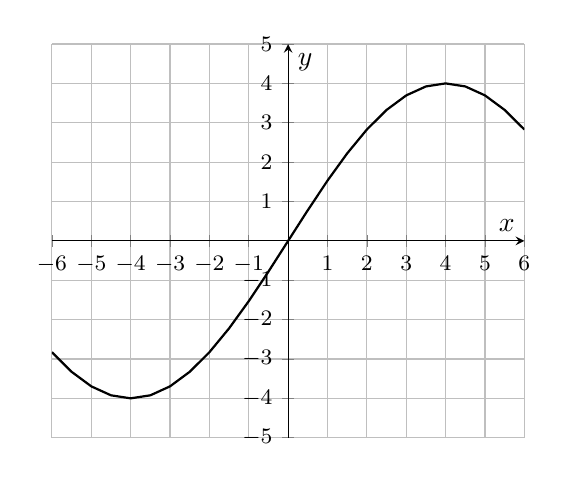
\begin{tikzpicture}
\begin{axis}[
	y=0.5cm,
    x=0.5cm,
	axis x line=middle,
	axis y line = middle,
	xmin=-6,xmax=6,
	ymin=-5,ymax=5,
    grid=both,
    xtick={-6,...,6},
    ytick={-5,...,5},
    xlabel=$x$,
    ylabel=$y$,
    tick label style={font=\footnotesize}
]
%\addplot[domain=0:1.9,mark=none, thick] {1-x};
%%\addplot[domain=0:1,mark=none, thick] {1};
%\addplot[domain=-2:0,mark=none, thick] {sqrt(1-(x+1)^2)+1};

\addplot[domain=-6:6,mark=none, thick] {4*sin(deg(2*pi*x/16))};
%\addplot[domain=2.07:3.97,mark=none, thick] {(x-2)^2+1};
%\addplot[domain=4.07:8,mark=none, thick] {cos(deg(x-4))+4};
%
%\addplot+[only marks, mark=*,  thick , black] coordinates {(2,3)};
%\addplot+[only marks, mark=o,  thick , black] coordinates {(2,1)(4,5)};



\node  at (axis cs:  6.1, 6.2) {\(y=g(x)\)};

\end{axis}
\end{tikzpicture}

\caption{Graph for Review Problem \ref{prob1}.}
\label{fig:prob1}

\end{figure}

\item Determine whether each cure shown in Figure \ref{fig:prob2} is the graph of a function. If it is, state the domain and range of the function.\label{prob2}


\begin{figure}[!h]
\centering
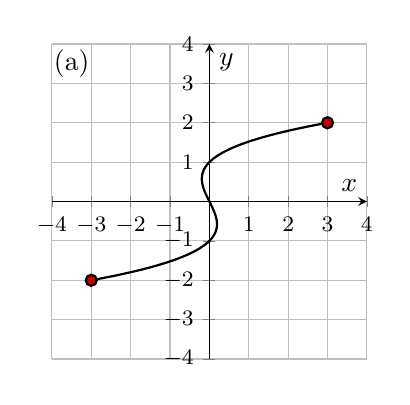
\begin{tikzpicture}
\begin{axis}[
	y=0.5cm,
    x=0.5cm,
	axis x line=middle,
	axis y line = middle,
	xmin=-4,xmax=4,
	ymin=-4,ymax=4,
    grid=both,
    xtick={-4,...,4},
    ytick={-4,...,4},
    xlabel=$x$,
    ylabel=$y$,
    tick label style={font=\footnotesize}
]
%\addplot[domain=0:1.9,mark=none, thick] {1-x};
%%\addplot[domain=0:1,mark=none, thick] {1};
%\addplot[domain=-2:0,mark=none, thick] {sqrt(1-(x+1)^2)+1};

\addplot[variable=\t, domain=-2:2,mark=none, thick,samples=100] (3/6*t*(t-1)*(t+1),t);
%\addplot[domain=2.07:3.97,mark=none, thick] {(x-2)^2+1};
%\addplot[domain=4.07:8,mark=none, thick] {cos(deg(x-4))+4};
%
\addplot+[only marks, mark=*,  thick , black] coordinates {(-3,-2)(3,2)};
%\addplot+[only marks, mark=o,  thick , black] coordinates {(2,1)(4,5)};



\node  at (axis cs:  -3.5,3.5) {(a)};

\end{axis}
\end{tikzpicture}
%
%
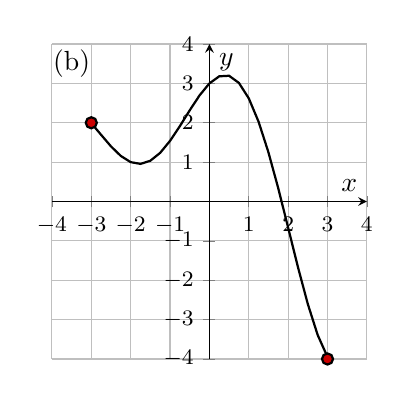
\begin{tikzpicture}
\begin{axis}[
	y=0.5cm,
    x=0.5cm,
	axis x line=middle,
	axis y line = middle,
	xmin=-4,xmax=4,
	ymin=-4,ymax=4,
    grid=both,
    xtick={-4,...,4},
    ytick={-4,...,4},
    xlabel=$x$,
    ylabel=$y$,
    tick label style={font=\footnotesize}
]
%\addplot[domain=0:1.9,mark=none, thick] {1-x};
%%\addplot[domain=0:1,mark=none, thick] {1};
%\addplot[domain=-2:0,mark=none, thick] {sqrt(1-(x+1)^2)+1};

%\addplot[variable=\t, domain=-2:2,mark=none, thick,samples=100] (3/6*t*(t-1)*(t+1),t);
\addplot[domain=-3:3,mark=none, thick] {((x+3)-1)*cos(deg(x))+1};
%\addplot[domain=4.07:8,mark=none, thick] {cos(deg(x-4))+4};
%
\addplot+[only marks, mark=*,  thick , black] coordinates {(-3,2)(3,-4)};
%\addplot+[only marks, mark=o,  thick , black] coordinates {(2,1)(4,5)};



\node  at (axis cs:  -3.5,3.5) {(b)};

\end{axis}
\end{tikzpicture}

\caption{Graph for Review Problem \ref{prob2}.}
\label{fig:prob2}

\end{figure}

\item Find the domain and range of the following functions. Write your answer in interval notation.
\begin{enumerate}


\item \(g(x) = \sqrt{16-x^2}\)

\item \(h(x) = 1+ \sin(x)\)

\item \(k(x) = \tan(2x)\)


\end{enumerate}

\item Suppose that the graph of \(f\) is given. Describe how the graphs of the following functions can be obtained from the graph of \(f\).
\begin{enumerate}

\item \(y = f(x)+6\)
\item \(y=f(x+6)\)
\item \(y = 1+2f(x)\)
\item \(y = f(x-2)-2\)

\end{enumerate}

\item The graph of \(f\) is shown in Figure \ref{fig:prob8}. Draw graphs of the following functions.\label{prob8}
\begin{enumerate}

\item \(y=f(x-1)\)
\item \(y = -f(x)\)
\item \(y = 1+f(x)\)
\item \(y = \frac{1}{2}f(x)-1\)

\end{enumerate}


\begin{figure}[!h]
\centering
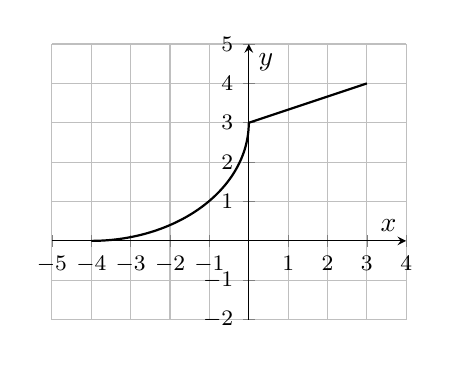
\begin{tikzpicture}
\begin{axis}[
	y=0.5cm,
    x=0.5cm,
	axis x line=middle,
	axis y line = middle,
	xmin=-5,xmax=4,
	ymin=-2,ymax=5,
    grid=both,
    xtick={-5,...,4},
    ytick={-2,...,5},
    xlabel=$x$,
    ylabel=$y$,
    tick label style={font=\footnotesize}
]
%\addplot[domain=0:1.9,mark=none, thick] {1-x};
%%\addplot[domain=0:1,mark=none, thick] {1};
%\addplot[domain=-2:0,mark=none, thick] {sqrt(1-(x+1)^2)+1};

\addplot[variable=\t, domain=-pi/2:0,mark=none, thick,samples=100] ({4*cos(deg(t))-4},{3*sin(deg(t))+3});
\addplot[domain=0:3,mark=none, thick] {x/3+3};

%\addplot[domain=-6:6,mark=none, thick] {4*sin(deg(2*pi*x/16))};
%\addplot[domain=2.07:3.97,mark=none, thick] {(x-2)^2+1};
%\addplot[domain=4.07:8,mark=none, thick] {cos(deg(x-4))+4};
%
%\addplot+[only marks, mark=*,  thick , black] coordinates {(2,3)};
%\addplot+[only marks, mark=o,  thick , black] coordinates {(2,1)(4,5)};



\node  at (axis cs:  6.1, 6.2) {\(y=g(x)\)};

\end{axis}
\end{tikzpicture}

\caption{Graph for Review Problem \ref{prob8}.}
\label{fig:prob8}

\end{figure}



\item If \(f(x) = \sqrt{x}\) and \(g(x) = \cos(x)\), find the following functions:
\begin{enumerate}

\item \(f \circ g\)
\item \(g \circ f\)
\item \(f \circ f\)
\item \(g \circ g\)

\end{enumerate}

\item Express the function \(F(x) = \frac{1}{\sqrt{x+\sqrt{x}}}\) as a composition of three functions.

\item The graph of \(f\) is given in Figure \ref{fig:prob19}. Find each limit, or explain why it does not exist. \label{prob19}

\begin{enumerate}
\item \(\displaystyle \lim_{x\rightarrow 2^+} f(x)\)
\item \(\displaystyle \lim_{x\rightarrow -3^+} f(x)\)
\item \(\displaystyle \lim_{x\rightarrow -3} f(x)\)
\item \(\displaystyle \lim_{x\rightarrow 4} f(x)\)
\item \(\displaystyle \lim_{x\rightarrow 0} f(x)\)
\item \(\displaystyle \lim_{x\rightarrow 2^-} f(x)\)

\end{enumerate}




\begin{figure}[!h]
\centering
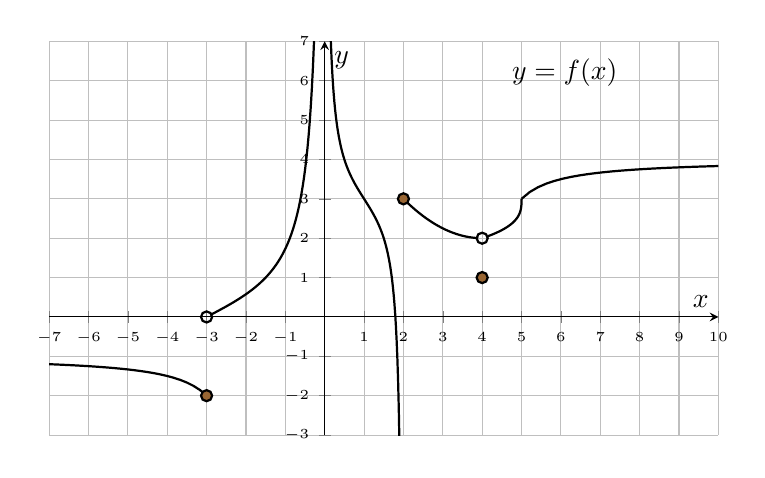
\begin{tikzpicture}
\begin{axis}[
	y=0.5cm,
    x=0.5cm,
	axis x line=middle,
	axis y line = middle,
	xmin=-7,xmax=10,
	ymin=-3,ymax=7,
    grid=both,
    xtick={-7,...,10},
    ytick={-3,...,7},
    xlabel=$x$,
    ylabel=$y$,
    tick label style={font=\tiny}
]
%\addplot[domain=0:1.9,mark=none, thick] {1-x};
%%\addplot[domain=0:1,mark=none, thick] {1};
%\addplot[domain=-2:0,mark=none, thick] {sqrt(1-(x+1)^2)+1};

\addplot[domain=-7:-3,mark=none, thick] {1/(x+2)-1};
\addplot[domain=-2.9:-.1,mark=none, thick,samples=100] {tan(deg(pi*(x+3)/6))};
\addplot[domain=.1:1.9,mark=none, thick,samples=100] {-tan(deg(pi*(x-1)/2))+3};
\addplot[domain=2:3.9,mark=none, thick] {1/4*(x-4)^2+2};
\addplot[variable=\t, domain=2.05:3,mark=none, thick,samples=100] ({(t-3)^3+5},{t});
\addplot[domain=5:10,mark=none, thick] {-1/(x-4)+4};

%
\addplot+[only marks, mark=*,  thick , black] coordinates {(-3,-2)(2,3)(4,1)};
\addplot+[only marks, mark=o,   thick , black] coordinates {(4,2)(-3,0)};



\node  at (axis cs:  6.1, 6.2) {\(y=f(x)\)};

\end{axis}
\end{tikzpicture}

\caption{Graph for Review Problem \ref{prob19}.}
\label{fig:prob19}

\end{figure}


\item Find the following limits.

\begin{enumerate}
\item \(\displaystyle \lim_{x\rightarrow 3}\ \frac{x^2-9}{x^2+2x-3}\)

\item \(\displaystyle \lim_{x\rightarrow -3}\ \frac{x^2-9}{x^2+2x-3}\)

\item \(\displaystyle \lim_{x\rightarrow 16}\ \frac{4-\sqrt{x}}{x-16}\)

\item \(\displaystyle \lim_{h\rightarrow 0}\ \frac{(h+1)^2-1}{h}\)

\end{enumerate}

\item Evaluate each limit, if it exists. If it does not exist, explain why.
\[
f(x) = \left\{
\begin{matrix}
\sqrt{-x}, & x<0\\
3-x, & 0\leq x <3\\
(x-3)^2, & x>3
\end{matrix}
\right.
\]

\begin{enumerate}
\item \(\displaystyle \lim_{x\rightarrow 0^+} f(x)\)
\item \(\displaystyle \lim_{x\rightarrow 0^-} f(x)\)
\item \(\displaystyle \lim_{x\rightarrow 0} f(x)\)
\item \(\displaystyle \lim_{x\rightarrow 3^-} f(x)\)
\item \(\displaystyle \lim_{x\rightarrow 3^+} f(x)\)
\item \(\displaystyle \lim_{x\rightarrow 3} f(x)\)

\end{enumerate}

\end{enumerate}

%\end{list}



\label{lastpage}

\end{document}